% Prof. Dr. Ausberto S. Castro Vera
% UENF - CCT - LCMAT - Curso de Ci\^{e}ncia da Computa\c{c}\~{a}o
% Campos, RJ,  2022
% Disciplina: An\'{a}lise e Projeto de Sistemas
% Aluno: 

\chapterimage{projeto.png} % Table of contents heading image
\chapter{Projeto do Sistema}

Com o objetivo de desenvolver um novo sistema para empresas que aviação que 
possuem varias sedes, apenas suficientemente parecido
com seu sistema atual para causar uma melhor transição e adaptação porém contendo todas as
melhorias necessárias e atendendo seus requisitos, foram realizadas uma série de atividades, divididas
em duas etapas: de planejamento e de análise.
Dentre as atividades realizadas estão o levantamento de requisitos, realização de entrevistas com
stakeholders para melhor compreensão e priorização dos requisitos, estudo de casos de uso para o
sistema, análise dos custos e benefícios do desenvolvimento deste novo sistema e um estudo sobre
sua viabilidade.
Concluiu-se que o sistema era viável e que seu 
desenvolvimento traria benefícios tanto tangíveis
quanto intangíveis para a empresa. 
Durante o cronograma estabelecido de um ano, serão
desenvolvidos o sistema de farmácia (que auxiliará no gerenciamento de vendas, estoque e finanças,
cadastro de funcionários, clientes e fornecedores e geração de relatórios), um website para venda
produtos online e um aplicativo de promoções e ofertas personalizadas para os clientes cadastrados.

\begin{figure}[!ht]
    \caption{Projeto do sistema}
    \centering
    
\includegraphics[width=5cm]{img.png}
\end{figure}
\section{Estrat\'{e}gia do Projeto}
Umas das estrategias é o desenvolvimento de um sistema totalmente 
personalizado em função do cliente, foi analisa um dos pontos importantes
para a escolha da opção dessa estrategia, entre eles:
\begin{itemize}
    \item A necessidade operacional é exclusiva
    \item O projeto tem um
          gerente altamente
          qualificado e uma
          metodologia comprovada
    \item O cronograma é flexível
\end{itemize}

\section{Arquitetura do Sistema}
Será utilizado a arquitetura de microsserviços baseado em 
múltiplos serviços e componentes para desenvolver uma estrutura modular,
permitiindo escalabilidade e independência dos módulos.

\begin{figure}[!ht]
    \caption{Visualização Microsserviço}
    \centering
    \includegraphics[width=15cm]{microsserviço.png}
\end{figure}


\section{Arquitetura do Hardware}
Os hardwares utilizados serão computadores 
e equipamentos nos quais 
os microsserviços são armazenados e executados. Estes 
servidores irão pertencer a provedores de infraestrutura em nuvem, 
como o Amazon Web Services, o Google Cloud Platform 
ou o Windows Azure. 

\begin{figure}[!ht]
    \caption{Opções de arquitetura para o microserviços}
    \centering
    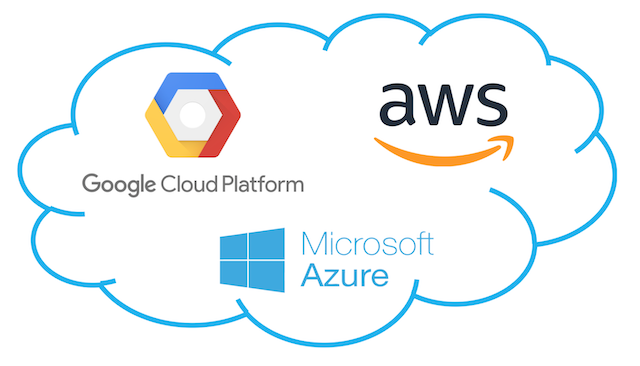
\includegraphics[width=10cm]{arquitetura.png}
\end{figure}

\section{Projeto de Interface}
A maioria dos usuários do nosso sistemas
interage com esses sistemas através de
interfaces gráficas, com interfaces baseadas em
texto, por isso se da muita importancia dentro dessa área.

\begin{figure}[!ht]
    \caption{Opções de arquitetura para o microserviços}
    \centering
    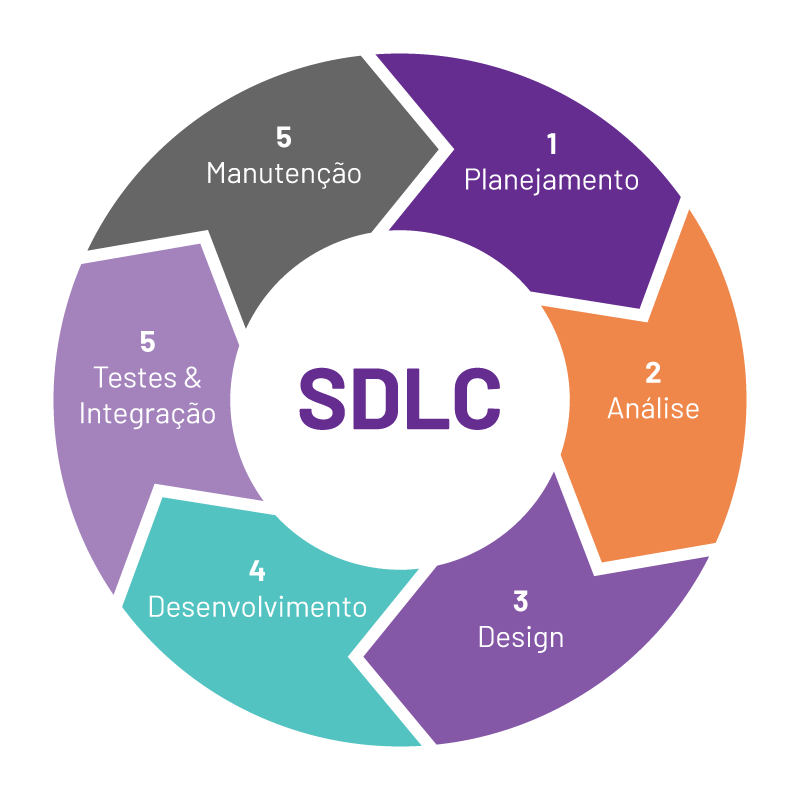
\includegraphics[width=10cm]{sdlc.png}
\end{figure}


